\documentclass{anstrans}
%%%%%%%%%%%%%%%%%%%%%%%%%%%%%%%%%%%
\title{Mixed Hybrid Finite Element Eddington Acceleration of Discrete Ordinates Source Iteration}
\author{Samuel S. Olivier*}

\institute{Department of Nuclear Engineering, Texas A\&M University, College Station, TX 77843}

\email{smsolivier@tamu.edu}


%%%% packages and definitions (optional)
\usepackage{graphicx} % allows inclusion of graphics
\usepackage{booktabs} % nice rules (thick lines) for tables
\usepackage{microtype} % improves typography for PDF

\usepackage{xspace}
\usepackage{siunitx}

\newcommand{\SN}{S$_N$\xspace}
\renewcommand{\vec}[1]{\bm{#1}} %vector is bold italic
\newcommand{\vd}{\bm{\cdot}} % slightly bold vector dot
\newcommand{\grad}{\vec{\nabla}} % gradient
\newcommand{\ud}{\mathop{}\!\mathrm{d}} % upright derivative symbol
\newcommand{\pderiv}[2]{\frac{\partial #1}{\partial #2}}
\newcommand{\dderiv}[2]{\frac{\ud #1}{\ud #2}}
\newcommand{\edd}{\langle \mu^2 \rangle} 

% add section on MHFEM system 
% order of accuracy of accelerated system 

\begin{document}
\section{Introduction}
	% Two of the most challenging computational tasks are radiation transport and hydrodynamics. 
	One of the most challenging computational tasks is simulating the interaction of radiation with matter. 
	A full description of a particle in flight includes three spatial variables ($x$,$y$ and $z$), two angular or direction of flight variables ($\mu =$ the cosine of the polar angle and $\gamma =$ the azimuthal angle), one energy variable ($E$) and one time variable ($t$). Numerical solutions require discretizing all seven variables leading to immense systems of algebraic equations. In addition, material properties can lead to vastly different solution behaviors making generalized numerical methods for radiation transport difficult to attain \cite{adams}. 

	% The conservation of mass, momentum and energy in hydrodynamics simulations leads to a hyperbolic system of partial differential equations dependent on the time derivatives of velocity and two state variables. This results in five variables but only three equations leading to the requirement of additional equations to reach problem closure \cite{hydro}. 

	% Radiation transport and hydrodynamics can be combined using operator splitting, where the radiation transport and hydrodynamics 

	Lawrence Livermore National Laboratory (LLNL) is developing a high--order radiation--hydrodynamics code. The hydrodynamics portion is discretized using the Mixed Hybrid Finite Element Method (MHFEM), where values are taken to be constant within a cell with discontinuous jumps at both cell edges \cite{mhfem}. MHFEM is particularly suited for hydrodynamics but not for radiation transport. This work seeks to develop an acceleration scheme capable of robustly reducing the number of iterations in Discrete Ordinates Source Iteration calculations while being compatible with MHFEM multiphysics.   

\section{Background}
	The steady--state, mono--energetic, isotropically--scattering, fixed--source Linear Boltzmann Equation in planar geometry is: 
		\begin{equation} \label{eq:bte}
			\mu \pderiv{\psi}{x}(x, \mu) + \Sigma_t(x) \psi(x,\mu) = 
			\frac{\Sigma_s(x)}{2} \int_{-1}^{1} \psi(x, \mu') d\mu' + \frac{Q(x)}{2}
		\end{equation}
	where $\mu = \cos\theta$ is the cosine of the angle of flight $\theta$ relative to the $x$--axis, $\Sigma_t(x)$ and $\Sigma_s(x)$ the total and scattering macroscopic cross sections, $Q(x)$ the isotropic fixed--source and $\psi(x, \mu)$ the angular flux \cite{adams}. This is an integro--differential equation due to the placement of the unknown, $\psi(x,\mu)$, under both a derivative and integral.

	The Discrete Ordinates (\SN) angular discretization sets $\mu$ to discrete values stipulated by an $N$--point Gauss quadrature rule. The scalar flux, $\phi(x)$, is then 
		\begin{equation} \label{eq:quad}
			\phi(x) = \int_{-1}^1 \psi(x, \mu) \ud\mu 
				\xrightarrow{\text{S}_N} \sum_{n=1}^N w_n \psi_n(x)
		\end{equation}
	where $\psi_n(x) = \psi(x,\mu_n)$ and $w_n$ are the quadrature weights corresponding to each $\mu_n$ \cite{llnl}. The \SN equations are then 
		\begin{equation} \label{eq:sn}
			\mu_n \dderiv{\psi_n}{x}(x) + \Sigma_t(x) \psi_n(x) = 
			\frac{\Sigma_s(x)}{2} \phi(x) + \frac{Q(x)}{2} 
		\end{equation}
	where $n = 1, 2, \dots, N$ and $\phi(x)$ is defined by Eq. \ref{eq:quad}. This is now a system of $N$ coupled, ordinary differential equations. 

	The Source Iteration (SI) solution method decouples the \SN equations by lagging the right hand side of Eq. \ref{eq:si}. In other words, 
		\begin{equation} \label{eq:si}
			\mu_n \dderiv{\psi_n^{\ell+1}}{x}(x) + \Sigma_t(x) \psi_n^{\ell+1}(x) = 
			\frac{\Sigma_s(x)}{2} \phi^{\ell}(x) + \frac{Q(x)}{2}, \ 1 \leq n \leq N
		\end{equation}
	where $\psi_n^\ell(x)$ is the solution from the $\ell^\text{th}$ iteration. Equation \ref{eq:si} represents $N$ independent ordinary differential equations. The iteration process begins with an initial guess for the scalar flux, $\phi^0(x)$. Equation \ref{eq:si} is then solved, using $\phi^0(x)$ on the right hand side, for the $\psi_n^1(x)$. $\phi^1(x)$ is then computed using Eq. \ref{eq:quad}.  
	This process is repeated until 
		\begin{equation} \label{eq:converg}
			\frac{\|\phi^{\ell+1}(x) - \phi^{\ell}(x)\|}{\|\phi^{\ell+1}(x)\|} < \epsilon
		\end{equation}
	where $\epsilon$ is a sufficiently small tolerance. 

	If $\phi^0(x) = 0$, then $\phi^\ell(x)$ is the scalar flux of particles that have undergone at most $\ell - 1$ collisions \cite{adams}. Thus, the number of iterations until convergence is directly linked to the number of collisions in a particle's lifetime. Typically, SI becomes increasingly slow to converge as the ratio of $\Sigma_s$ to $\Sigma_t$ approaches unity and the amount of particle leakage from the system goes to zero. SI is slowest in large, optically thick systems with small losses to absorption. In full radiation transport simulations each iteration could involve solving for hundreds of millions of unknowns. To minimize computational expense, acceleration schemes must be developed to rapidly increase the rate of convergence of SI. 

	Fortunately, the regime where SI is slow to converge is also the regime where Diffusion Theory is most accurate. A popular method for accelerating SI is Diffusion Synthetic Acceleration (DSA) where each source iteration involves both a transport sweep and a diffusion solve. DSA requires carefully differencing the \SN and diffusion steps in a consistent manner to prevent instability in highly scattering media with coarse spatial grids \cite{alcouffe,morel}. DSA is not applicable in the setting of this presentation due to the incompatibility of MHFEM and \SN and the increased computational expense of solving consistently differenced diffusion. A new acceleration method is needed that avoids the consistency pitfall of DSA. 

\section{Eddington Acceleration}
	The zeroth and first angular moments of Eq. \ref{eq:bte} are 
		\begin{subequations} 
		\begin{equation} \label{eq:zero}
			\dderiv{}{x} J(x) + \Sigma_a(x) \phi(x) = Q(x) 
		\end{equation} 
		\begin{equation} \label{eq:first}
			\frac{\ud}{\ud x} \edd(x) \phi(x) + \Sigma_t(x) J(x) = 0  
		\end{equation}
		\end{subequations}
	where $J(x) = \int_{-1}^{1} \mu \ \psi(x, \mu) \ud \mu$ is the current and 
		\begin{equation} \label{eq:eddington} 
			\edd(x) = \frac{\int_{-1}^1 \mu^2 \psi(x, \mu) \ud \mu}{\int_{-1}^1 \psi(x, \mu) \ud \mu}
			% \xrightarrow{\text{S}_N} \frac{\sum_{n=1}^N \mu_n^2 w_n\psi_n(x)}{\sum_{n=1}^N w_n \psi_n(x)} 
		\end{equation}
	the Eddington factor. In \SN, the Eddington factor is 
		\begin{equation} \label{eq:edd_sn}
			\edd(x) = \frac{\sum_{n=1}^N \mu_n^2 w_n\psi_n(x)}{\sum_{n=1}^N w_n \psi_n(x)}.
		\end{equation}
	Note that no approximations have been made to arrive at Eqs. \ref{eq:zero} and \ref{eq:first}. The Eddington factor is the true angular flux weighted average of $\mu^2$ and therefore Eqs. \ref{eq:zero} and \ref{eq:first} are just as accurate as Eq. \ref{eq:bte}. 

	This formulation is beneficial because Eq. \ref{eq:zero} is a conservative balance equation and---if $\edd(x)$ is known---the moment equations' system of two first--order, ordinary differential equations can be solved directly with well--established methods. However, computing $\edd(x)$ requires already knowing the angular flux. 

	The proposed acceleration scheme is: 
		\begin{enumerate}
			\item Compute $\psi_n(x)$ with \SN and an arbitrary spatial discretization
			\item Compute $\edd(x)$ with Eq. \ref{eq:edd_sn}
			\item Interpolate $\edd(x)$ onto the MHFEM grid 
			\item Solve the moment equations for $\phi(x)$ with the preconditioned $\edd(x)$ using MHFEM. 
		\end{enumerate}
	This process is one source iteration consisting of an \SN transport step to compute the Eddington factor and an MHFEM acceleration step to compute $\phi(x)$. The scalar flux from the acceleration step is used in the right hand side of Eq. \ref{eq:si} and steps 1--4 are repeated until the acceleration step's $\phi(x)$ converges according to Eq. \ref{eq:converg}.  

	Acceleration occurs because the Eddington factor is a weak function of angular flux. This means that even poor angular flux solutions can accurately approximate the Eddington factor. In addition, the moment equations model the contributions of all scattering events at once, reducing the dependence on source iterations to introduce scattering information. The solution from the acceleration step is then an approximation for the full flux and not the $\ell - 1$ collided flux as it was without acceleration. 

	In addition to acceleration, this scheme allows the \SN equations and moment equations to be solved with different spatial discretizations. \SN can be spatially discretized using normal methods such as Linear Discontinuous Galerkin or Diamond Differencing while the moment equations can be solved on the same grid as the hydrodynamics. 
	% operator split iteration, computationally economic to use moment equations 

	% This method differs from DSA in that two solutions are generated: one from \SN and one from the moment equations and that the \SN and acceleration steps do not have to be consistently differenced. The solution of the moment equations will be used because the moment equations are conservative while \SN is not. 

% \section{Diamond Differenced \SN}
% 	The Diamond Differenced (DD) \SN equations corresponding to Eq. \ref{eq:sn} are 
% 		\begin{equation} \label{eq:dd}
% 			\frac{\mu_n}{h_i}\left(\psi_{n,i+1/2} - \psi_{n,i-1/2}\right)
% 				+ \Sigma_{t,i} \psi_{n,i} = \frac{\Sigma_{s,i}}{2}\sum_{n'=1}^N \psi_{n',i}w_{n'}
% 				+ \frac{Q_i}{2}
% 		\end{equation}
% 	where $\psi_{n,i\pm1/2} = \psi_n(x_{i\pm1/2})$ is the cell edge angular flux and $\Sigma_{t,i} = \Sigma_t(x_i)$, $\Sigma_{s,i} = \Sigma_s(x_i)$ and $Q_i = Q(x_i)$ the cell averaged total cross section, scattering cross section and fixed source. The $x_{i\pm1/2}$ are the cell edge locations of cell $i$ of cell width $h = x_{i+1/2} - x_{i-1/2}$. In DD, the cell centered angular flux is taken to be the average of the adjacent cell edge angular fluxes: 
% 		\begin{equation} \label{eq:auxDD}
% 			\psi_{n,i} = \frac{1}{2} \left(\psi_{n,i+1/2} + \psi_{n,i-1/2}\right)
% 		\end{equation}


\section{Results}
	As a proof of concept for Eddington acceleration, a Diamond Differenced \SN code was created along with an MHFEM solver for Eqs. \ref{eq:zero} and \ref{eq:first}. The test problem of steady--state, one--group, isotropically--scattering, fixed--source radiation transport in slab geometry with a reflecting left boundary and vacuum right boundary was used to compare unaccelerated, Eddington accelerated, and DSA S$_8$ SI with 100 spatial cells. 

	\begin{figure} % replace 't' with 'b' to force it to be on the bottom
		\centering
		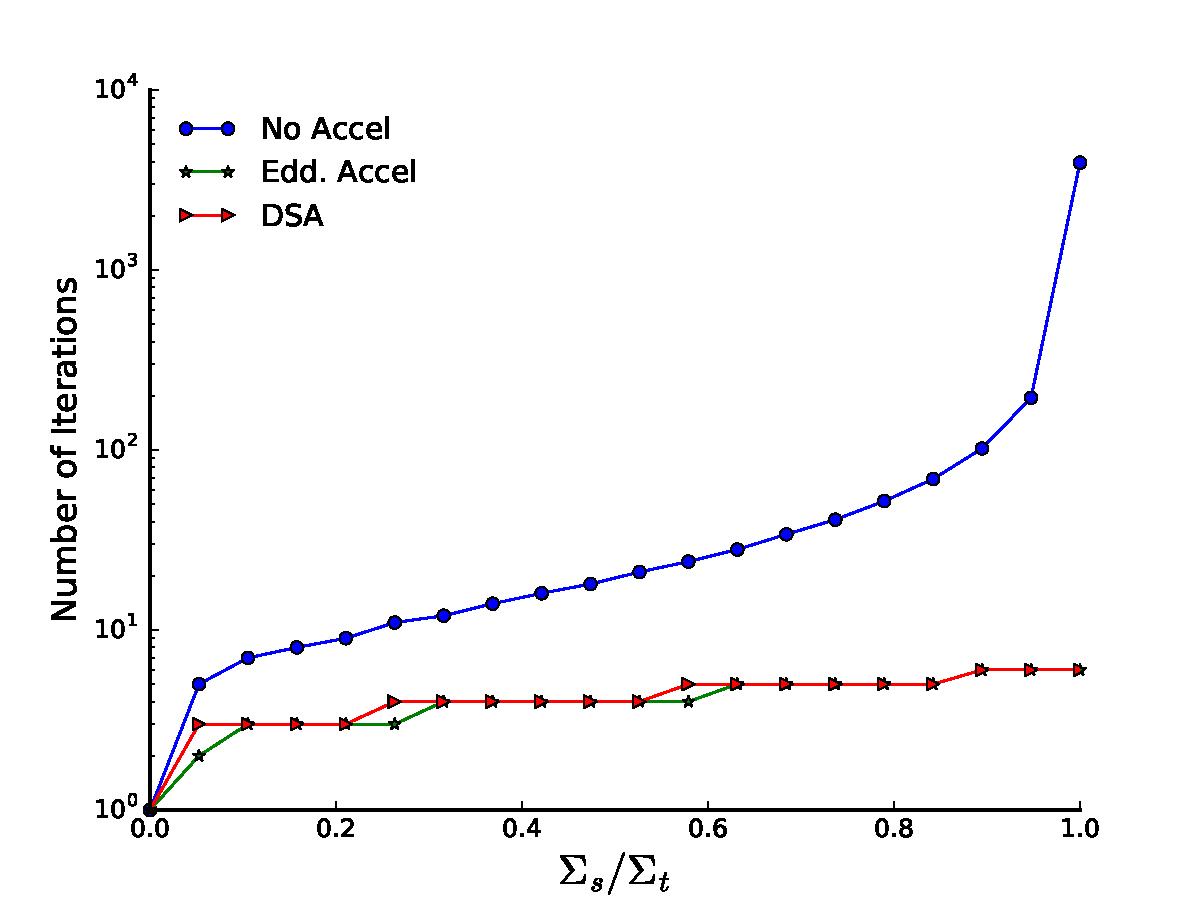
\includegraphics[width=8.5cm]{accel.pdf}
		\caption{A comparison of the number of iterations until convergence for unaccelerated, Eddington accelerated, and DSA S$_8$ SI. }
		\label{fig:comparison}
	\end{figure}

	Figure \ref{fig:comparison} shows the number of iterations until the convergence criterion in  Eq. \ref{eq:converg} was met with $\epsilon = \num{1e-6}$ for varying ratios of $\Sigma_s$ to $\Sigma_t$. Aside from $\Sigma_s/\Sigma_t = 0$ where acceleration is not possible, the ratio of unaccelerated to Eddington accelerated iterations ranges between 2.5 and 750. This suggests that acceleration is occurring and that Eddington acceleration does not just do twice the amount of work in each iteration. 

	\begin{figure}
		\centering
		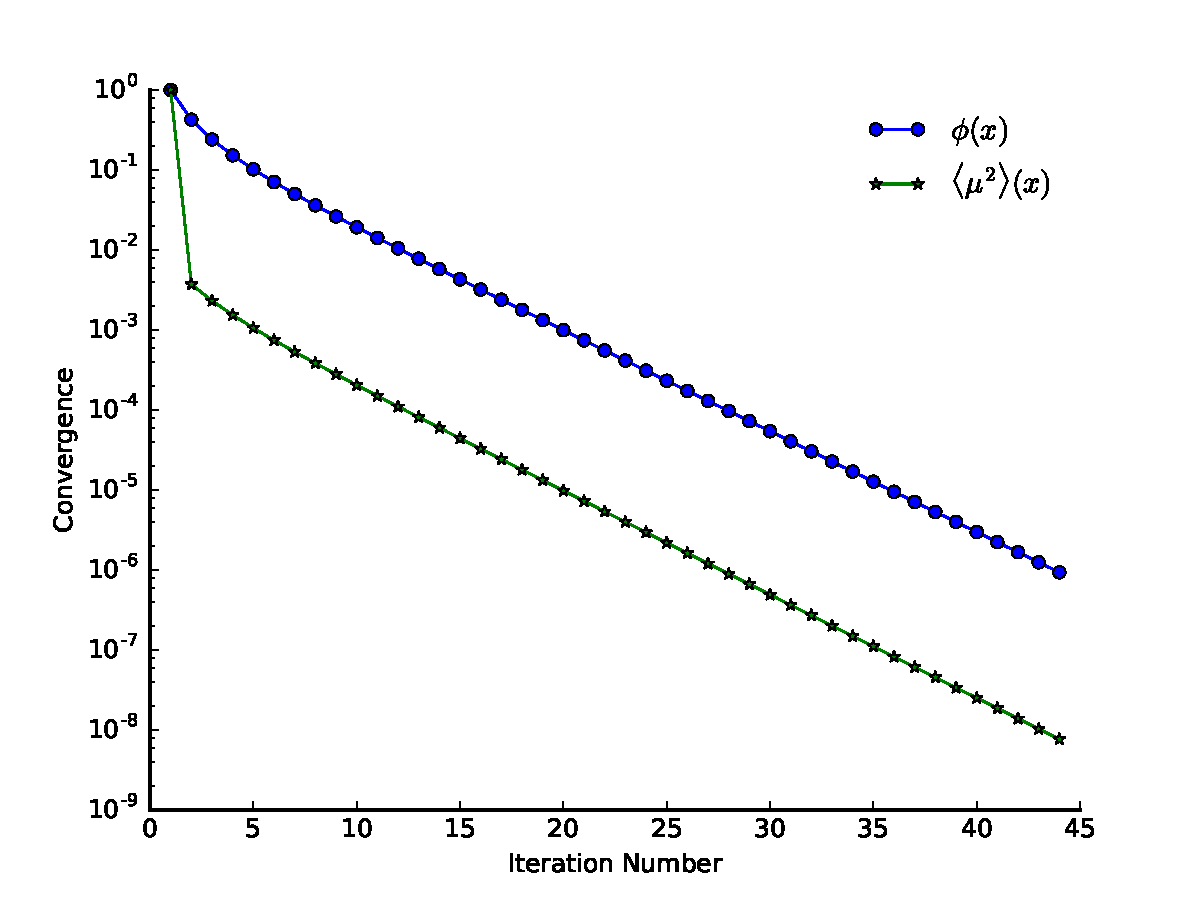
\includegraphics[width=8.5cm]{eddCon_si.pdf}
		\caption{The convergence rate of $\phi(x)$ compared to $\edd(x)$ for unaccelerated S$_8$. }
		\label{fig:conv_si}
	\end{figure}

	Figure \ref{fig:conv_si} shows the unaccelerated convergence criterion 
		\begin{equation}
			\frac{\|f^{\ell+1} - f^{\ell}\|}{\|f^{\ell+1}\|}
		\end{equation}
	as a function of iteration number for $f = \phi(x)$ and $f = \edd(x)$. The large drop in the convergence criterion between the first and second iterations supports the claim that $\edd(x)$ is a weak function of angular flux as it quickly converges despite a less convergent angular flux. When compared to Fig. \ref{fig:conv_edd}, a plot of the convergence criterion versus number of iterations for Eddington accelerated S$_8$, it is clear that Eddington acceleration transfers the fast rate of convergence of $\edd(x)$ to $\phi(x)$. 

	\begin{figure}
		\centering
		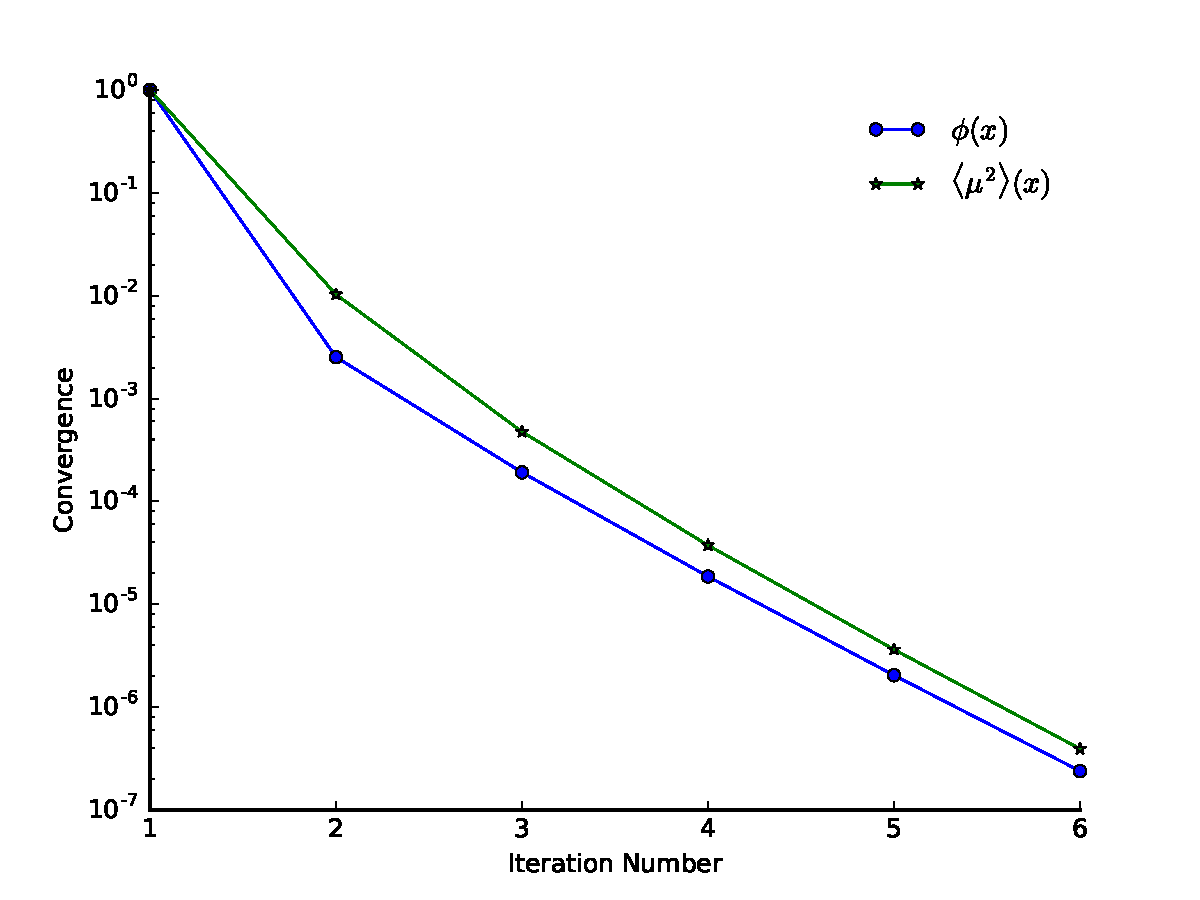
\includegraphics[width=8.5cm]{eddCon_mu.pdf}
		\caption{The convergence rate of $\phi(x)$ compared to $\edd(x)$ for Eddington accelerated S$_8$.}
		\label{fig:conv_edd}
	\end{figure}

	% add convergence rate of phi v edd 
	% include discussion on acceleration v just doing 2 times as much work. ie actual acceleration is happening 

\section{Conclusions}
	The proposed acceleration scheme successfully accelerated S$_8$ source iteration calculations in slab geometry for a wide range of $\Sigma_s/\Sigma_t$. In the pure scattering regime ($\Sigma_s = \Sigma_t$), source iteration was accelerated by a factor of 750. This scheme is especially suited for multiphysics applications because the transport and acceleration steps do not need to be consistently differenced. In addition, the acceleration step produces a conservative solution that is computationally inexpensive compared to a transport sweep. Future work that will also be presented is the application of Eddington acceleration to Linear Discontinuous Galerkin discretized \SN. 

% \section{Acknowledgments}

\bibliographystyle{ans}
\bibliography{bibliography.bib}
\end{document}